% !TEX root = document.tex

\chapter{\label{chap:sdf3}WebDSL in SDF3}

  In computer science, parsing is the process of analyzing a piece of text according to a grammar, and converting the textual representation to a more structured represation that is convenient for other processes such as a compiler or interpreter.

  In this chapter we discuss the definition of the WebDSL grammar in SDF3, a meta-DSL in Spoofax for syntax definition. Currently, the WebDSL grammar is defined in SDF2, the predecessor of SDF3. The goal of defining the WebDSL grammar in SDF3 instead of SDF2 is to serve as a large case study for SDF3, while allowing the WebDSL parser to benefit from the regular updates of SDF3, compared to the deprecated SDF2.

  We start by giving a brief introduction to parsing in general and introducing the SDF3 language. Then, we discuss the migration of the WebDSL syntax from SDF2 to SDF3 and we end this chapter by elaborating on the disambiguation of the WebDSL SDF3 grammar without the use of post-parse filters.

  \section{\label{sec:parsing}Introduction to LR Parsing}

    Every programming language can be described by a grammar that specifies what a syntactically correct program looks like. Given a specific program, this grammar can be used to analyze whether the program belongs to the language described by the grammar. A parser is a piece of software that is able to recognize whether a program belongs to the grammar described by the parser. Additionally, parsers create a structured representation of the input program, derived from the textual representation.
    
    In this thesis, we will focus on \textit{LR parsers}. LR stands for Left-to-right Rightmost-derivation, meaning that an LR parser reads the input from left to right and produces a rightmost (bottom-up) derivation. Knuth \citeyear{knuth1965translation} presents an LR parsing algorithm which is able to parse most languages that can be described by a context-free grammar.

    Before an LR parser can parse an input stream, it must also receive a parse table that describes a context-free grammar. In practice, the parse tables are usually generated from a syntax definition. \Cref{fig:example-cfg-with-parse-table} shows an example of a context-free grammar describing a small language that features addition and multiplication. The parse table describes a push-down automaton that represents the LR parser. Using this parse table, an LR parser can build a parse tree as shown in \cref{fig:example-parse-tree}. A parse tree, or an Abstract Syntax Tree (AST) that we will discuss in \cref{subsec:sdf3} is a more structured way of representing a program, that can be used by other components of a compilation chain to analyze and transform the program.

    \begin{figure}[h]
      \begin{subfigure}[b]{0.25\textwidth}
        \centering
        \begin{align*}
        S &\longrightarrow E\\
        E &\longrightarrow E + T\\
        E &\longrightarrow T\\
        T &\longrightarrow T * F\\
        T &\longrightarrow F\\
        F &\longrightarrow x
        \end{align*}
        \caption{\label{fig:example-cfg-with-parse-table-cfg}}
      \end{subfigure}
      \begin{subfigure}[b]{0.75\textwidth}
        \centering
        \begin{tabular}{ c || c | c | c | c || c | c | c | c }
          State & \multicolumn{4}{c||}{Action} & \multicolumn{4}{c}{Goto} \\
          \hline
          & + & * & x & \$ & $S$ & $E$ & $T$ & $F$ \\
          \hline
          0 & & & $S(4)$ & & & 1 & 2 & 3 \\
          \hline
          1 & $S(5)$ & & & $Accept$ & & & & \\
          \hline
          2 & $R(E_T)$ & $S(6)$ & & $R(E_T)$ & & & & \\
          \hline
          3 & $R(T_F)$ & $R(T_F)$ & & $R(T_F)$ & & & & \\
          \hline
          4 & $R(F_x)$ & $R(F_x)$ & & $R(F_x)$ & & & & \\
          \hline
          5 & & & $S(4)$ & & & & 7 & 3 \\
          \hline
          6 & & & $S(4)$ & & & & & 8 \\
          \hline
          7 & $R(E_{E+T})$ & $S(6)$ & & $R(E_{E+T})$ & & & & \\
          \hline
          8 & $R(T_{T*F})$ & $R(T_{T*F})$ & & $R(T_{T*F})$ & & & & \\
        \end{tabular}
        \caption{\label{fig:example-cfg-with-parse-table-tbl}}
      \end{subfigure}
      \caption{\label{fig:example-cfg-with-parse-table}Example context-free grammar with its parse table}
    \end{figure}

    \begin{figure}
      \centering
      \begin{tikzpicture}
        \node {$S$}
          child {node {$E$}
            child {node {$T$}
              child {node {$T$}
                child {node {$F$}
                  child {node {$x$}}
                }
              }
              child {node {$*$}}
              child {node {$F$}
                child {node {$x$}}
              }
            }
          };
      \end{tikzpicture}
      \caption{\label{fig:example-parse-tree}An example of a parse tree for the input "$x * x$"}
    \end{figure}

    LR parsers cannot handle ambiguous context-free grammars. The parse tables of ambiguous context-free grammars contain multiple state transitions for certain states and input tokens. The Generalized LR (GLR) parsing algorithm by Rekers (\citeyear{Rekers1992}), is able to handle such parse tables and as a result is able to handle all context-free grammars. Visser \citeyear{Visser97SGLR} introduced Scannerless GLR (SGLR) parsing. As opposed to LR and GLR parsers, SGLR parsers do not have a separate lexing and parsing phase, but instead merge these through the use of grammars that are defined in terms of single characters.

    \subsection{\label{subsec:sdf3}SDF3}

      Syntax Definition Formalism 3 (SDF3) \autocite{VollebregtKV12,AmorimV20} is a meta-language in the Spoofax language workbench that makes use of the SGLR parsing algorithm. It is the latest version of the syntax definition formalism SDF \autocite{HeeringHKR89,Visser97}. Language engineers are able to define context-free grammars in SDF3, which are transformed into parse tables and used by the JSGLR2\footnote{\url{https://github.com/metaborg/jsglr}} parsing algorithm. JSGLR2 \autocite{Denkers2018} is the successor of the JSGLR algorithm; an implementation of the SGLR parsing algorithm in Java.

      SDF3 is the successor of SDF2, in which the WebDSL syntax is currently defined. Souza Amorim and Visser \citeyear{AmorimV20} argue that the SDF3 syntax is more similar to other grammar formalisms such as EBNF.

      A syntax definition in SDF3 is a declarative specification of syntactic sorts and their productions. \Cref{fig:sdf3-sorts-and-productions-syntax} shows an example grammar features a language that supports multiplication and addition of integers. The SDF3 definition must define a start-symbol that specifies what a syntactically valid program looks like. In our example, every program that can be derived from the \texttt{Start} sort, is a valid program. \textbf{Line 11} contains the first production of the specification. It startes that the sort \texttt{Start} can be derived by deriving something of the sort \texttt{Expr}. The identifier behind the dot in the production (\texttt{Expr} in this case) declares the constructor in the AST. \Cref{fig:example-AST-1} shows the AST of an example input, according to the SDF3 specification of \cref{fig:sdf3-sorts-and-productions-syntax}. \textbf{Line 12-14} defines the productions of the expression sort. It defines that an expression is either two expressions with a plus or asterix in between, or it is something of the sort \texttt{Lit}. The production of literal sort on \textbf{line 16} references the lexical sort \texttt{INT}. Lexical sorts do not appear in the AST with constructors, but instead are parsed into a string. The lexical sort \texttt{INT} is defined on \textbf{line 22} with the regular expression \texttt{[0-9]+}, describing one or more characters in the range of 0 to 9. Finally, the production describing the built-in concept of \texttt{LAYOUT} on \textbf{line 23} states that a space, tab, carriage return and line feed character are layout (whitespace) characters and do not have to be parsed.

      \Cref{fig:example-AST-1} shows the abstract syntax tree of an example input for the SDF3 specification of \cref{fig:sdf3-sorts-and-productions-syntax}. In the Spoofax Language Workbench, abstract syntax trees are described in the Annotated Terms Format (ATerm) \autocite{BrandJKO00}.

      \begin{figure}
        \begin{minted}[firstline=1]{\sdfthree}
  module ThesisTest

  context-free start-symbols
    Start

  context-free sorts
    Start Expr Lit

  context-free syntax
    Start.Expr = <<Expr>>

    Expr.Add = <<Expr> + <Expr>>
    Expr.Mul = <<Expr> * <Expr>>
    Expr.Lit = <<Lit>>

    Lit.Int = <<INT>>

  lexical sorts
    INT

  lexical syntax
    INT    = [0-9]+
    LAYOUT = [\ \t\n\r]
        \end{minted}
        \caption{\label{fig:sdf3-sorts-and-productions-syntax}An SDF3 specification of a language that allows addition and multiplication of integers.}
      \end{figure}

      \begin{figure}
        \begin{subfigure}[b]{0.5\textwidth}
          \centering
          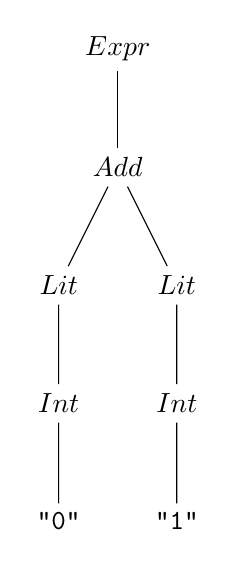
\begin{tikzpicture}
            \node {$Expr$}
              child {node {$Add$}
                child {node {$Lit$}
                  child {node {$Int$}
                    child {node {\texttt{"0"}}}
                  }
                }
                child {node {$Lit$}
                  child {node {$Int$}
                    child {node {\texttt{"1"}}}
                  }
                }
              };
          \end{tikzpicture}
          \caption{\label{fig:example-AST-1-ast}}
        \end{subfigure}
        \begin{subfigure}[b]{0.5\textwidth}
          \begin{minted}[firstline=1]{text}
Expr(
  Add(
    Lit(Int("0")),
    Lit(Int("1"))
  )
)
          \end{minted}
          \caption{\label{fig:example-AST-1-aterm}}
        \end{subfigure}
        \caption{\label{fig:example-AST-1}The AST and ATerm representation of the expression \texttt{0 + 1} according to the SDF3 specification of \cref{fig:sdf3-sorts-and-productions-syntax}}
      \end{figure}

      In addition to the basics as explained in the previous paragraph, SDF3 supports features such as injections, optional sorts and repetition to enhance the language engineers productivity. \cref{fig:sdf3-syntax-injection-repetition-optional} shows the SDF3 specification of \cref{fig:sdf3-sorts-and-productions-syntax}, but now enhanced with injections, repitition and optional sorts. \Cref{fig:example-aterm-injections-etc} shows the ATerm of the input \texttt{0 + 0; 1 * -1}. The repetition on \textbf{line x} of \cref{fig:sdf3-syntax-injection-repetition-optional} allows multiple expressions in a list, delimited by a semicolon. The injection on \textbf{line 14} allows a literal to be derived in the place of an expression, effectively omitting the \texttt{Lit(...)} constructor in the AST. Lastly, the optional minus sign of \textbf{line 16 and 18} allows negative integers to be parsed by this language. The AST contains \texttt{Some(...)} and \texttt{None()} constructors for the optional sorts.
        
      \begin{figure}
        \begin{minted}[firstline=1]{\sdfthree}
  module m

  context-free start-symbols
    Start
  
  context-free sorts
    Start Expr Lit Minus
  
  context-free syntax
    Start.Exprs = <<{Expr "; "}+>>
  
    Expr.Add = <<Expr> + <Expr>>
    Expr.Mul = <<Expr> * <Expr>>
    Expr     = Lit
  
    Lit.Int = <<Minus?> <INT>>
  
    Minus.Minus = <->
  
  lexical sorts
    INT
  
  lexical syntax
    INT    = [0-9]+
    LAYOUT = [\ \t\n\r]
        \end{minted}
        \caption{\label{fig:sdf3-syntax-injection-repetition-optional}An SDF3 specification of a language that allows addition and multiplication of integers, showcasing injections, repetition and optional sorts.}
      \end{figure}

      \begin{figure}
        \begin{minted}[firstline=1]{text}
  Exprs([
    Add(
      Int(None(), "0"),
      Int(None(), "0")
    ),
    Mult(
      Int(None(), "1")
      Int(Some(Minus()), "1")
    )
  ])
        \end{minted}
        \caption{\label{fig:example-aterm-injections-etc}The ATerm of input \texttt{0 + 0; 1 * -1} according to the SDF3 specification of \cref{fig:sdf3-syntax-injection-repetition-optional}}
      \end{figure}

      \subsubsection{\label{subsubsec:sdf3-disambiguation}Disambiguation}

        The simple grammar described by the SDF3 specification of \cref{fig:sdf3-sorts-and-productions-syntax} is functional, but is ambiguous. For example, the input \texttt{1 + 2 + 3} can be parsed as \texttt{(1 + 2) + 3} or as \texttt{1 + (2 + 3)}. The process of altering and annotating the grammar such that this there is only one way of parsing this, is called disambiguation. The example listed in the previous section (\cref{fig:example-cfg-with-parse-table}) contains a grammar with expressions, terms and factors that is inherently unambiguous. However, disambiguating a grammar by introducing new sorts and productions is tedious and time consuming. SDF3 provides multiple options for disambiguating a grammar.

        First of all, SDF3 provides the \texttt{\{bracket\}} annotation, allowing the developer to disambiguate the program himself. To clarify, the input \texttt{1 + (2 + 3)} is not valid according to our grammar, because the "(" and ")" symbols are not part of the grammar. If we add the production \texttt{Expr = "(" Expr ")" \{bracket\}}, SDF3 allows brackets around arbitrary expressions without it introducing new AST nodes.

        Reject rules allow language engineers to filter derivations. A reject rule is simple a regular production, followed by the \texttt{\{reject\}} annotation. For example, appending our grammar with the rule \texttt{Expr = <<Expr> + <Expr>> \{reject\}} makes the set of valid derivations of \texttt{Expr} smaller, namely by disallowing any construction described by the right-hand side of the reject rule.

        Another possibility for disambiguating SDF3 grammars is by indicating the associatibity, either as annotation or using priority groups. If we add the annotation \texttt{\{left\}} to the production that specifies addition, \texttt{1 + 2 + 3} is no longer ambiguous but instead will always be parsed as \texttt{(1 + 2) + 3}. It is also possible to declare the associativity in groups. \Cref{fig:sdf3-syntax-disambiguation} contains such groups. \textbf{Line 8} shows that both addition and subtraction are left associative, and in the same group. The input \texttt{1 + 2 - 3 + 4} will now be parsed as \texttt{((1 + 2) - 3) + 4}, whereas declaring the associativity annotation on both rules instead of the group would still make this input ambiguous.

        \begin{figure}
          \begin{minted}[firstline=2]{\sdfthree}
  module m
  context-free syntax
    Expr.Mul = <<Expr> * <Expr>>
    Expr.Add = <<Expr> + <Expr>>
    Expr.Sub = <<Expr> - <Expr>>

  context-free priorities
    {left: Expr.Mul} >
    {left: Expr.Add Expr.Sub }
          \end{minted}
          \caption{\label{fig:sdf3-syntax-disambiguation}An SDF3 specification of a simple language with disambiguation rules.}
        \end{figure}

        \Cref{fig:sdf3-syntax-disambiguation} also shows the declaration of priorities. In the example, multiplication has priority (e.g. binds tighter) over addition and subtraction. This results in the input \texttt{1 + 2 - 3 * 4} being parsed as \texttt{(1 + 2) - (3 * 4)}.

        SDF3 also provides the option of indexed priorities in the form of \texttt{p1 i .> p2}. This can be explained intuitively as the subterm with index \texttt{i} of production \texttt{p1} may not be derived by production \texttt{p2}. In our example, the rule \texttt{Expr.Add <0> .> Expr.Mul} would imply that the left-hand side of an addition may never be a multiplication.

        Lastly, SDF3 provides the ability to disambiguate through the use of post-parse filters annotated by \texttt{\{prefer\}} and \texttt{\{avoid\}}. When the parser encounters an ambiguous input, it will continue parsing and store all possibilities. At the end of parsing, it will use the annotations to prune the multiple ASTs according to these annotations. The \texttt{\{prefer\}} and \texttt{\{avoid\}} annotations are working but deprecated in the current version of SDF3 and will be removed in the future. Using the post-parse filters makes the disambiguation less transparent than using the other methods described in this section.

  \section{\label{sec:webdsl-grammar}WebDSL Grammar Specification}

    The current grammar of WebDSL is specified in SDF2, the predecessor of SDF3.

    The WebDSL grammar specification consists of <> files with <> productions in total.
    
    Parts of the syntax are deprecated but still mainainted for backwards compatibility reasons.

    Some productions added for the sake of autocompletion.

    Reason to switch to SDF3:
    \\- Modern spoofax does not support SDF2 anymore
    \\- Good case study for performance
    \\- Good case study for prefer/avoid 
    \\- Necessary to efficiently interact with Statix: signature generator

  \section{\label{sec:sdf2-to-sdf3}Migration from SDF2 to SDF3}

    There is a tool to migrate SDF2 specifications to SDF3 specifications but it does not work in all cases. Some work needs to be done to prepare the SDF2 specification for the migration, and some work needs to be done on the resulting SDF3 specification to make sure it is as usable as the old SDF2 specification.

    \subsection{\label{subsec:preparing-webdsl-sdf2}Preparing the WebDSL SDF2 definition for migration}

      The SDF2 to SDF3 migration tool does not accept "sorts" sections.
      \\\\Alternations must be removed from the SDF2 specification. Solution is to introduce a separate sort for the alternation:
      \\\\Before:
      \\("B" | "C") -> A \{cons("A")\}
      \\\\After:
      \\BorC -> A    \{cons("A")\}
      \\"B"  -> BorC \{cons("B")\}
      \\"C"  -> BorC \{cons("C")\}
      \\\\Restrictions (both context-free and lexical) produce an error during transformation and must be manually copied.
      \\\\Mixed languages and parameterized imports are currently not supported in SDF3, so WebDSL code cannot be mixed with Stratego/Java code in the new SDF3 syntax definition.
      \\\\Mixed languages were only used in the compiler, except for HQL which is used in WebDSL code. Fortunately, the HQL syntax is not used elsewhere and could be transformed to be a part of the WebDSL syntax natively.

    \subsection{\label{subsec:manual-tweaking-sdf3}Manual Tweaking of Generated WebDSL SDF3}

      \subsubsection{Missing and duplicate constructors}

        In SDF3, the constructors are a much more key part of the productions than in SDF2, where constructors are defined as a \texttt{cons("MyConstructor")} annotation on the production. In the WebDSL SDF2 definition, some constructors were missing and there were many duplicate constructors that denoted alternative syntax for the same construct, essentially providing syntactic sugar.
        
        In the newly generated SDF3, duplicate constructors had to be changed, in order for them to be unique. Additionally, missing constructors had to be added, preferably even for injections for a reason we will touch on later in \cref{sec:preparation-for-statix}.

      \subsubsection{Priority chains}

        To indicate priority amongst context-free productions, both SDF2 and SDF3 use the concept of priority chains, but the SDF2 variant requires a repitition of the production inside the chain, whereas SDF3 uses a reference to the sort with corresponding constructor. This causes the SDF2 priority chains to not be migrated to the SDF3 priority chains.
        
        The only way to tackle this issue is to manually re-enter the priority chains in SDF3.

      \subsubsection{Transferring comments}

        Of a lesser importance, but highly recommended for the readability of a syntax definition is the comments, that are parsed as layout and are therefore not tranfered to the generated SDF3 files. Again, there is no way around this and they have to be manually transferred.

      \subsubsection{Template productions}

        A major change in SDF3 compared to SDF2 are template productions, that allow for nice pretty printing and syntactic code completion. The productions in the generated SDF3 files are all template productions, but do not have the proper surrounding layout and indentation because there is no way to extract this information from the SDF2 source. This had to be manually added to the generated SDF3 productions where applicable.

      \subsubsection{Deeply embedding HQL}

        Previously, the syntax definition of HQL was a standalone definition, and was used in the WebDSL SDF2 through parameterized imports. SDF3 has no support for this feature, so as discussed in \cref{subsec:preparing-webdsl-sdf2}, the language has to be transformed to be a part of the WebDSL syntax.
        
        Deeply embedding the HQL syntax in the WebDSL syntax causes some errors to arise on duplicate names of sorts and constructors, this had to be fixed manually.

  \section{\label{sec:preparation-for-statix}Preparation for Statix}

    With the intention to use Statix for implementing the WebDSL static analyses, the grammar sorts and constructors have strict requirements. Statix is a strongly typed language and requires all input to adhere to the declared sorts and constructors.

    \subsection{\label{subsec:sorts-in-statix}Sorts and Constructors in Statix}

      Statix takes an abstract syntax tree as input.
      \\\\In the signature definition of Statix rules, it must be stated what the input and output sorts are. The implementation of the rules are defined over the constructors that belong to the sorts in the rule's signature.
      \\\\Demo: Left top a few SDF3 productions, right top an abstract syntax tree, bottom statix sorts, constructors and a few rules.
      \\\\All sorts and constructors that rules are defined over, have to be defined in the Statix code. In our case, a complete redefinition of all sorts and constructors in the Statix code is necessary to statically analyze the all WebDSL language features.
      \\\\Unlike SDF3 and Stratego, Statix is statically typed and does not support injections or polymorphism in its constructors, which leaves some abstract syntax trees generated by the parser unable to serve as input for static analysis.

    \subsection{\label{subsec:statix-signature-generator}Statix Signature Generator}

      As mentioned and demonstrated in \cref{subsec:sorts-in-statix}, Statix requires a definition of the constructors and sorts of the language to be analyzed. This definition exists in SDF3, but is not compatible with the Statix semantics since no injections are allowed. To prevent manual redefinition of the sorts in Statix code, the Statix Signature Generator is developped. This tool takes the SDF3 definition as input, and generates importable Statix files that contain the sorts and constructors from the syntax definition. For the Statix Signature Generator to work properly, Additional well-formedness requirements exist for the SDF3 definition.

      \subsubsection{Explicitly Declare Sorts}

        The parser generator that takes an SDF3 definition as input, is able to extract the sorts names from productions. Unfortunately, this is not the case for the Statix Signature generator so all sorts used in productions must be declared explicitly in \texttt{context-free sorts} and \texttt{lexical sorts} blocks.
        \\\\TO-DO: Find reason and describe here
        \\\\TO-DO: Example here with before and after with context-free and lexical sort blocks

      \subsubsection{Injections}

        With the semantics of Statix' constructors and sorts, it is not possible to model injections.
        \\\\TO-DO: Example of injection here and impossibility of modelling in Statix
        \\\\The Statix Signature Generator deals with simple injections (from one sort to one sort) by explicating the injections, making a more verbose version of the constructors and sorts.
        \\\\TO-DO: Example here of simple injection explicated
        \\\\Even though this functions properly, it is hard to read in the Statix rules. For this reason, we changed the WebDSL SDF3 to contain less injections by inserting constructors with descriptive names where injections were.
        \\\\TO-DO: Show result

      \subsubsection{\label{subsubsec:sdf3-optional-sorts}Optional Sorts}

        As mentioned in \cref{subsec:sdf3-syntax}, SDF3 has built-in support for optional sorts, resulting in \texttt{Some(\_)} and \texttt{None()} terms.
        \\\\The resulting terms cannot be translated to Statix signatures, since this would mean a lot of duplicate Some and None constructors belonging to different sorts.
        \\\\To resolve this challenge, the SDF3 definition must be altered make the Some and None constructors unique per sort. This leads to a much more verbose syntax definition:
        \\\\TO-DO: Example here with two syntax definitions and resulting ASTs: one with built-in optional sorts, other with verbose optional sorts.

      \subsubsection{Disambiguation}

        As mentioned in \cref{subsec:sdf3-syntax}, ambiguous code fragments lead to abstract syntax trees with the \texttt{amb(\_, \_)} term. Similar to optional sorts, this cannot be translated to Statix and therefore it is crucial that the syntax is disambiguated properly.
        \\\\Next to this, the \texttt{prefer} and \texttt{avoid} annotations for disambiguation were heavily used in the WebDSL SDF2 definition. The annotations are supported in SDF3, but the support is likely to be dropped in a future release.
        \\\\For the two reasons listed above, we reimplemented disambiguation through a combination of multiple SDF3 features. This process is explained in \cref{sec:webdsl-sdf3-disambiguation}.

  \section{\label{sec:webdsl-sdf3-disambiguation}Disambiguation}
  
    Since the \texttt{amb(\_,\_)} constructor is not declarable in Statix, having an ambiguity in the AST leads to the analysis not executing. This increases the need for disambiguation.
    \\\\Challenges and solutions:
    \begin{itemize}
      \item Keywords in WebDSL: SDF3 template options not optimal.
      \item String interpolation: Convert to one String constructor with a list of parts.
      \item Optional separators: In SDF2 multiple productions could have the same constructor, in SDF3 multiple constructors make for an increase in reject and desugaring rules.
      \item Optional alias vs. cast expression: use non-transitive priority rule.
    \end{itemize}
